\documentclass[a4paper,12pt]{exam}
	\usepackage{graphicx}
	\usepackage[utf8]{inputenc}
	\usepackage[T1]{fontenc}
	\usepackage{listings}
	\usepackage{color}
	\usepackage{amsmath}
	\usepackage{enumerate}
	\usepackage{caption}
	\usepackage{subcaption}
	\definecolor{dkgreen}{rgb}{0,0.6,0}
	\definecolor{gray}{rgb}{0.5,0.5,0.5}
	\definecolor{mauve}{rgb}{0.58,0,0.82}

	\lstset{frame=tb,
	  language=Python,
	  aboveskip=3mm,
	  belowskip=3mm,
	  showstringspaces=false,
	  columns=flexible,
	  basicstyle={\small\ttfamily},
	  numbers=none,
	  numberstyle=\tiny\color{gray},
	  keywordstyle=\color{blue},
	  commentstyle=\color{dkgreen},
	  stringstyle=\color{mauve},
	  breaklines=true,
	  breakatwhitespace=true
	  tabsize=3
	}

\begin{document}
\begingroup 
	  \bf \Large Mecânica Clássica I\\
	  \indent \normalsize André Del Bianco Giuffrida
	\endgroup
	\\ \quad
	\\
	Uma particula desloca-se ao longo da parábola
	\[ y^2 = 4f_{0}^{2} -4f_0 x\] \\
	Afim de simplificar vamos utilizar $f_0 = 1$  \\
		\begin{figure}[h]
			\centering
			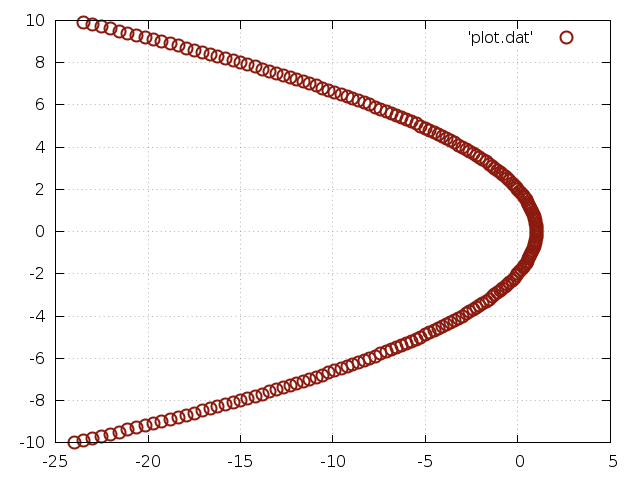
\includegraphics[scale=0.3]{2o0.png}
			\caption{Movimento - Coordenadas retangulares}
		\end{figure}

		podemos visualizar aqui a distância em funçao do angulo $\theta$
		como sabemos que a particula possui velocidade constante, podemos escrever
		
		\[ \vec{r} = x \hat x + \sqrt{4-4x} \hat y\]
		Como :
		\[ \vec{v} = \dot x \hat x + \dot y \hat y = cte \]
		\[\dot x = 1 - \frac{y \dot y}{2}  \quad \quad \text{e} \quad \quad \dot y = -\frac{\dot x}{\sqrt{1-x}}\]
		Já em Coordenadas polares temos a velocidade $\vec{v}$ definida por:
		\[\vec{v} = \dot r \hat r + r \dot \theta \hat \theta = \text{cte}\]
		...
		
\end{document}		
